\documentclass[a0paper,36pt]{extarticle}

\usepackage[a0paper, portrait,
  top=95mm, bottom=18mm,
  left=22mm, right=22mm]{geometry}

\usepackage[utf8]{inputenc}
\usepackage[T1]{fontenc}
\usepackage[english]{babel}
\usepackage{lmodern}
\usepackage{amsmath,amssymb}
\usepackage{graphicx}
\usepackage{booktabs}
\usepackage{multicol}
\usepackage{xcolor}
\usepackage{tikz}
\usepackage{eso-pic}
\usepackage{mdframed}
\usepackage{parskip}
\usepackage{setspace}
\usepackage{array}
\usepackage{caption}
\usepackage{calc}
\usepackage{pifont}

% --- Kolory motywu ---
\definecolor{pwrviolet}{RGB}{92,45,145}
\definecolor{pwrdark}{RGB}{40,20,70}
\definecolor{accentyellow}{RGB}{220,180,0}
\definecolor{blockbg}{RGB}{247,244,252}
\definecolor{alertbg}{RGB}{255,251,230}
\definecolor{darktext}{RGB}{25,25,25}
\definecolor{mutedtext}{RGB}{80,80,80}

% --- Tło: szablon Digital Horizons ---
\AddToShipoutPictureBG{%
  \AtPageLowerLeft{%
    \includegraphics[width=\paperwidth,height=\paperheight,keepaspectratio=false]%
      {Digital Horizons- format A0, vertically.png}%
  }%
}

% --- Blok z tytułem ---
\mdfdefinestyle{blockstyle}{%
  backgroundcolor=blockbg,
  linecolor=pwrviolet,
  linewidth=2pt,
  roundcorner=6pt,
  innertopmargin=20pt,
  innerbottommargin=22pt,
  innerleftmargin=18pt,
  innerrightmargin=18pt,
  skipabove=16pt,
  skipbelow=14pt
}
\mdfdefinestyle{alertstyle}{%
  backgroundcolor=blockbg,
  linecolor=accentyellow,
  linewidth=3pt,
  roundcorner=6pt,
  innertopmargin=20pt,
  innerbottommargin=22pt,
  innerleftmargin=18pt,
  innerrightmargin=18pt,
  skipabove=16pt,
  skipbelow=14pt
}

\newcommand{\pblock}[2]{%
  \begin{mdframed}[style=blockstyle]
    \noindent{\color{white}\colorbox{pwrviolet}{%
      \parbox{\dimexpr\linewidth-2\fboxsep\relax}{%
        \vspace{8pt}\Large\bfseries\strut\MakeUppercase{#1}\strut\vspace{8pt}}}}%
    \vspace{12pt}\par
    \setstretch{1.6}\Large\color{darktext}#2
  \end{mdframed}}

\newcommand{\ablock}[2]{%
  \begin{mdframed}[style=alertstyle]
    \noindent{\color{white}\colorbox{pwrviolet}{%
      \parbox{\dimexpr\linewidth-2\fboxsep\relax}{%
        \vspace{8pt}\Large\bfseries\strut\MakeUppercase{#1}\strut\vspace{8pt}}}}%
    \vspace{12pt}\par
    \setstretch{1.6}\Large\color{darktext}#2
  \end{mdframed}}

\setlength{\columnsep}{24pt}
\setlength{\itemsep}{6pt}
\pagestyle{empty}
\captionsetup{font=normalsize,labelfont=bf,labelsep=period}

% =============================================================
\begin{document}

% --- TYTUŁ ---
\begin{center}
  {\fontsize{64}{64}\selectfont\bfseries\color{pwrdark}%
    Comparison of Deep Learning Models}\\[10pt]
  {\fontsize{64}{64}\selectfont\bfseries\color{pwrdark}%
    for Multi-Organ CT Segmentation}\\[10pt]
  {\fontsize{64}{64}\selectfont\bfseries\color{pwrdark}%
    Under Limited Data Conditions}\\[22pt]
  {\fontsize{42}{50}\selectfont\color{pwrviolet}\bfseries
    Jakub Ciszewski}\\[14pt]
  {\fontsize{32}{40}\selectfont\color{mutedtext}
    Politechnika Warszawska}\\[10pt]
  {\fontsize{30}{38}\selectfont\color{mutedtext}
    \texttt{jakub.ciszewski.dokt@pw.edu.pl}}
\end{center}

\vspace{4mm}
\noindent\textcolor{pwrviolet}{\rule{\linewidth}{2pt}}
\vspace{2mm}

% =============================================================
% GÓRNA CZĘŚĆ — 3 kolumny tekstowe
% =============================================================
\begin{multicols}{3}
\raggedcolumns

% -------- KOLUMNA 1 --------
\pblock{Introduction}{%
  Automatic organ segmentation in computed tomography (CT) is a key
  component of modern medical image analysis, supporting applications
  such as \textbf{radiotherapy planning}, surgical navigation, and
  quantitative assessment.

  Deep learning methods, particularly CNNs such as U-Net and its
  variants, have become the standard for biomedical image segmentation.
  Transformer-based architectures and foundation models have been
  proposed to improve generalization.

  However, many approaches are developed on \textbf{large datasets},
  while real-world clinical scenarios often involve \textbf{limited
  annotated data}.
}

\pblock{Aim}{%
  Compare selected deep learning architectures for
  \textbf{multi-organ segmentation in abdominal CT}
  under \textbf{limited data conditions}.
}

\pblock{Dataset}{%
  \begin{itemize}\setlength{\itemsep}{8pt}
    \item[$\triangleright$] \textbf{18 abdominal CT scans} from a
      public medical imaging dataset
    \item[$\triangleright$] Annotated organs: \textbf{liver, spleen,
      kidneys, stomach, gallbladder, esophagus}
    \item[$\triangleright$] Split: \textbf{14 training} /
      \textbf{4 validation} cases
    \item[$\triangleright$] \textbf{5-fold cross-validation} for robust
      evaluation
  \end{itemize}
}

\pblock{Methods}{%
  Evaluated architectures:
  \begin{itemize}\setlength{\itemsep}{8pt}
    \item[$\bullet$] \textbf{U-Net} — 2D, 2.5D, and 3D variants
    \item[$\bullet$] \textbf{nnU-Net} — self-configuring framework
    \item[$\bullet$] \textbf{Swin-UNETR} — transformer-based
    \item[$\bullet$] \textbf{MedNeXt} — recent architecture
    \item[$\bullet$] \textbf{TotalSegmentator} — pretrained benchmark
  \end{itemize}
  \medskip
  All models used a \textbf{unified preprocessing pipeline}.
  Performance evaluated with the \textbf{Dice Similarity Coefficient
  (DSC)}, ensuring a fair comparison across architectures.
}

\pblock{Future Work}{%
  \begin{itemize}\setlength{\itemsep}{8pt}
    \item[$\triangleright$] Improving segmentation of small and
      low-contrast organs
    \item[$\triangleright$] Evaluation on larger multi-center datasets
    \item[$\triangleright$] Incorporating multimodal or temporal data
    \item[$\triangleright$] Exploring hybrid CNN--Transformer models
  \end{itemize}
}

% -------- KOLUMNA 2 --------
\columnbreak

\pblock{Results}{%
  \textbf{nnU-Net} and \textbf{UNet-2.5D} achieved the highest overall
  segmentation performance (\textbf{mean Dice $\approx$ 0.61}), with
  \textbf{UNet-2D} performing nearly identically.

  \medskip
  \textbf{TotalSegmentator} achieved competitive results ($\approx$~0.60),
  particularly for large, well-defined organs (e.g., liver, stomach).
  However, performance dropped significantly for selected classes
  (e.g., right kidney, aorta), likely due to label inconsistencies
  or dataset mismatch.

  \medskip
  \textbf{Transformer-based models} (Swin-UNETR, MedNeXt) showed clearly
  reduced performance (mean Dice $\approx$ 0.36 and 0.24), indicating
  high sensitivity to limited training data.
}

\pblock{Size-Dependent Effect}{%
  A clear relationship between \textbf{organ size} and segmentation
  performance was observed:
  \begin{itemize}\setlength{\itemsep}{8pt}
    \item[$\uparrow$] \textbf{Large structures} (liver, stomach) —
      consistently high Dice across all models (often $>$ 0.7)
    \item[$\downarrow$] \textbf{Small / low-contrast structures}
      (esophagus, aorta) — consistently low performance across models
  \end{itemize}
  \medskip
  This indicates a strong \textbf{size-dependent bias}: larger organs
  are learned more reliably, while small and low-contrast structures
  remain challenging regardless of architecture.
}

\pblock{Limitations}{%
  \begin{itemize}\setlength{\itemsep}{8pt}
    \item[$\triangleright$] Very small dataset (18 CT scans)
    \item[$\triangleright$] Possible label inconsistencies
      (TotalSegmentator)
    \item[$\triangleright$] No hyperparameter optimization per model
    \item[$\triangleright$] Limited evaluation of small structures
  \end{itemize}
}

\ablock{Key Takeaways}{%
  \begin{itemize}\setlength{\itemsep}{8pt}
    \item[\ding{228}] Best performance: nnU-Net / UNet-2.5D
      ($\approx$ 0.61 Dice)
    \item[\ding{228}] Largest drop for small organs (esophagus, aorta)
    \item[\ding{228}] Pretrained models sensitive to label mismatch
    \item[\ding{228}] Model simplicity outperforms complexity in
      low-data regime
  \end{itemize}
}

\pblock{Per-Organ Dice — All Methods}{%
  \begin{center}
    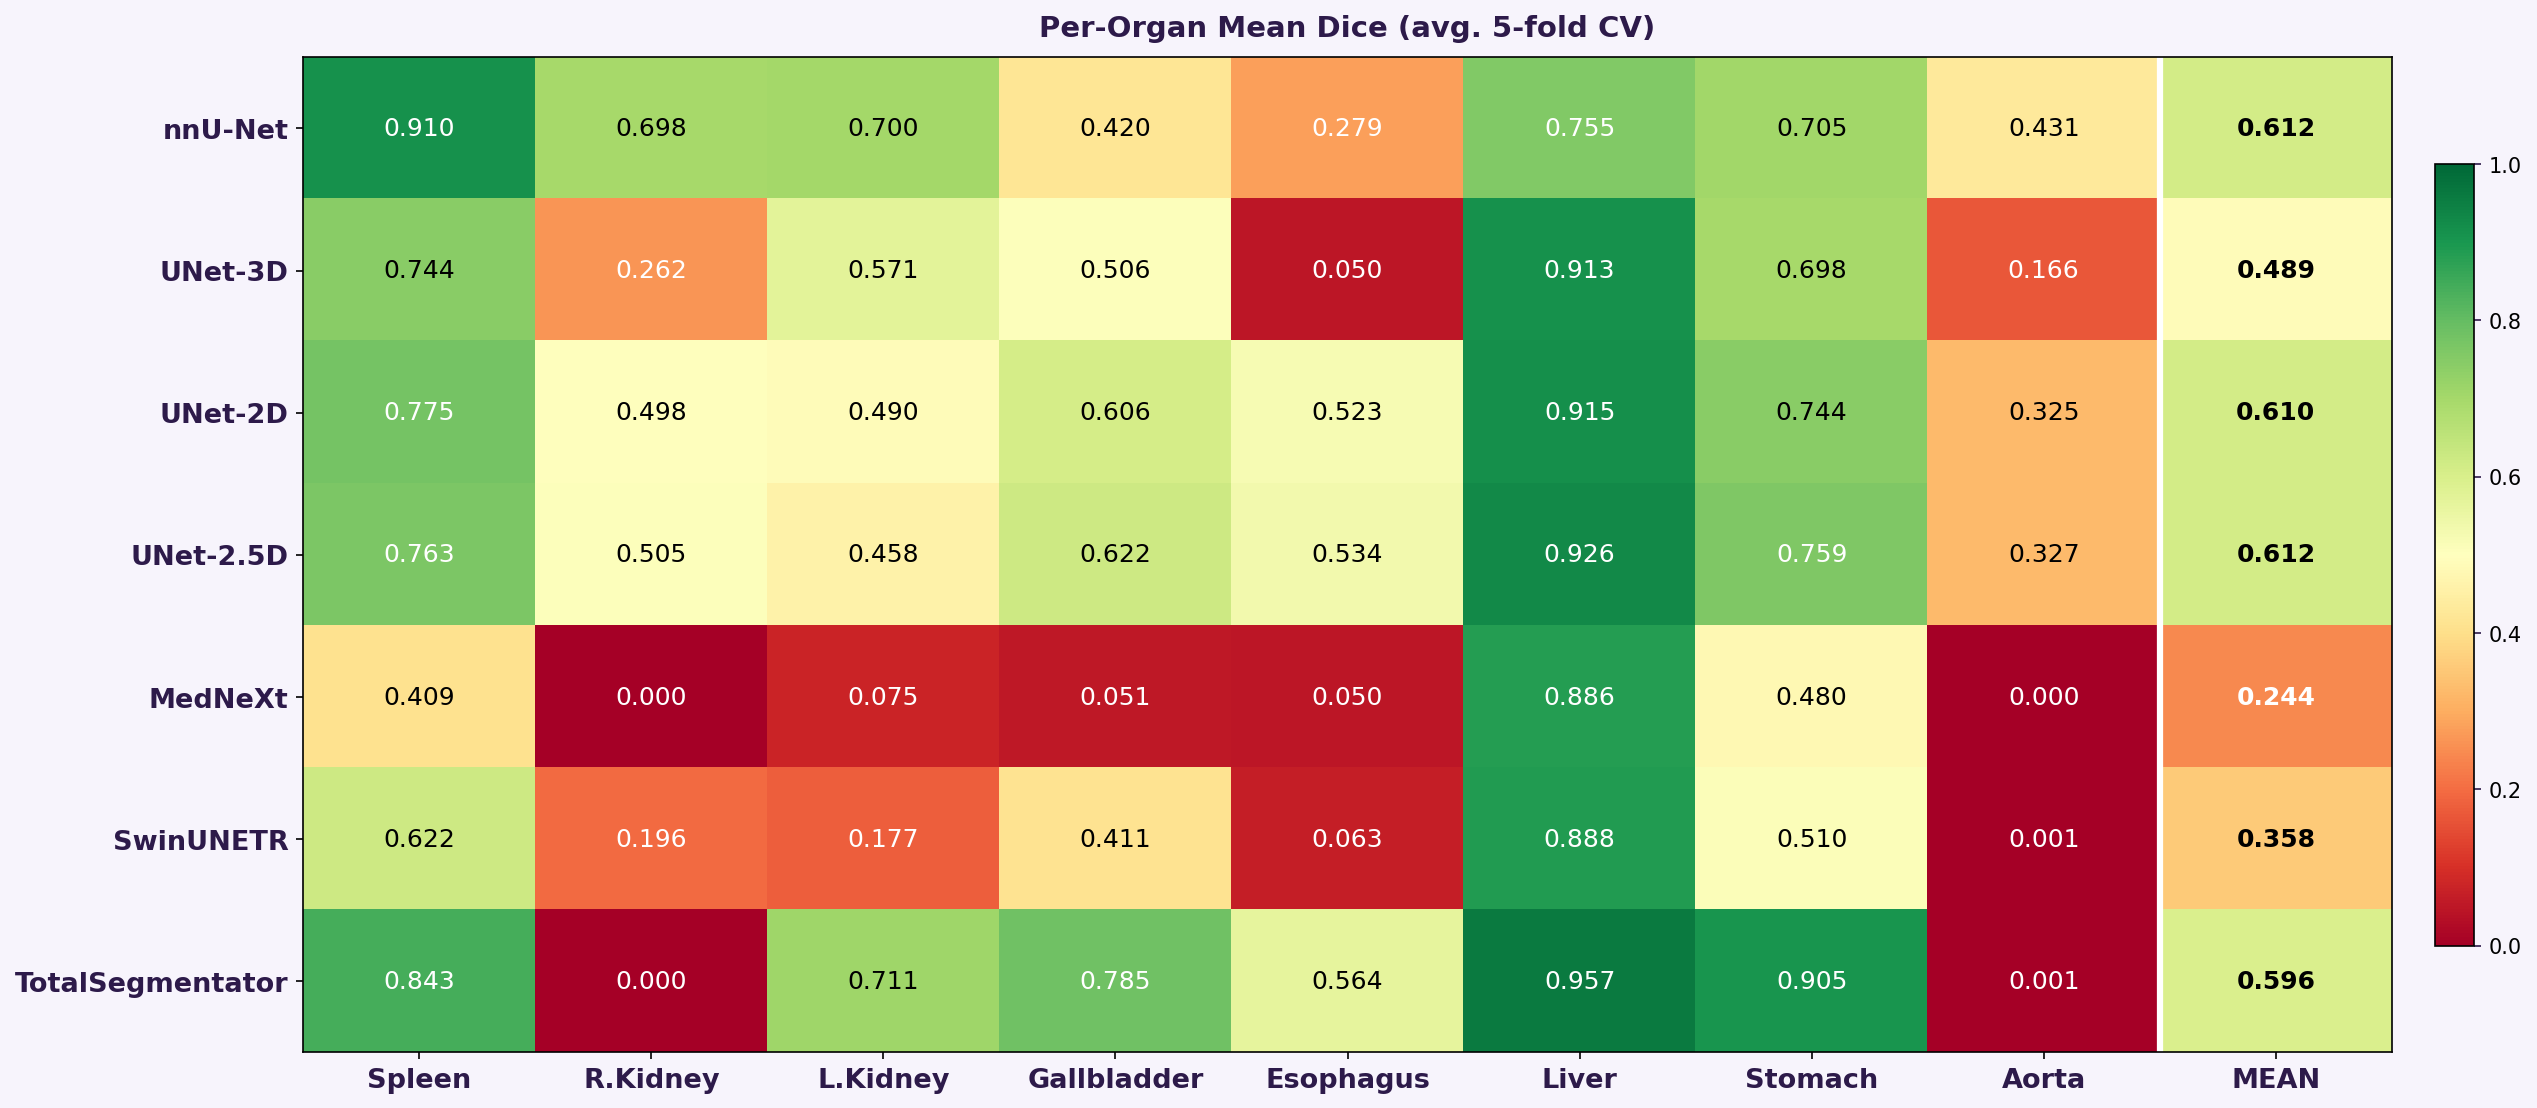
\includegraphics[width=\linewidth]{multiorgan_full_comparision.png}
  \end{center}
}

% -------- KOLUMNA 3 --------
\columnbreak

\pblock{Discussion}{%
  Model performance is influenced not only by \textbf{architecture}
  but also by \textbf{organ characteristics} and potential
  \textbf{label inconsistencies}.

  \smallskip
  Advanced architectures \textbf{degrade significantly in small-data
  settings}, while simpler CNN-based approaches and nnU-Net remain
  \textbf{stable and competitive}. Failures of pretrained models on
  specific organs highlight the importance of \textbf{dataset alignment}.
}

\ablock{Conclusion}{%
  \textbf{nnU-Net} and \textbf{UNet-2.5D} provide the most robust
  performance for multi-organ CT segmentation under limited data
  conditions.

  \medskip
  \begin{itemize}\setlength{\itemsep}{8pt}
    \item[\checkmark] Organ size and anatomical complexity strongly
      influence segmentation quality
    \item[\checkmark] Classical CNN-based approaches remain highly
      competitive
    \item[\checkmark] Transformer-based models require larger datasets
      to achieve strong performance
  \end{itemize}
}

\pblock{Practical Implications}{%
\begin{itemize}\setlength{\itemsep}{8pt}
  \item[$\triangleright$] nnU-Net and UNet-2.5D are reliable choices
    for clinical scenarios with limited annotated data
  \item[$\triangleright$] Special care is required for small organs,
    where segmentation errors are most likely
  \item[$\triangleright$] Pretrained models should be used with caution
    due to potential label mismatches
  \item[$\triangleright$] Simpler architectures may offer better
    cost–performance trade-offs in real-world deployments
\end{itemize}
}


\pblock{All Methods — Mean Dice Comparison}{%
  \begin{center}
    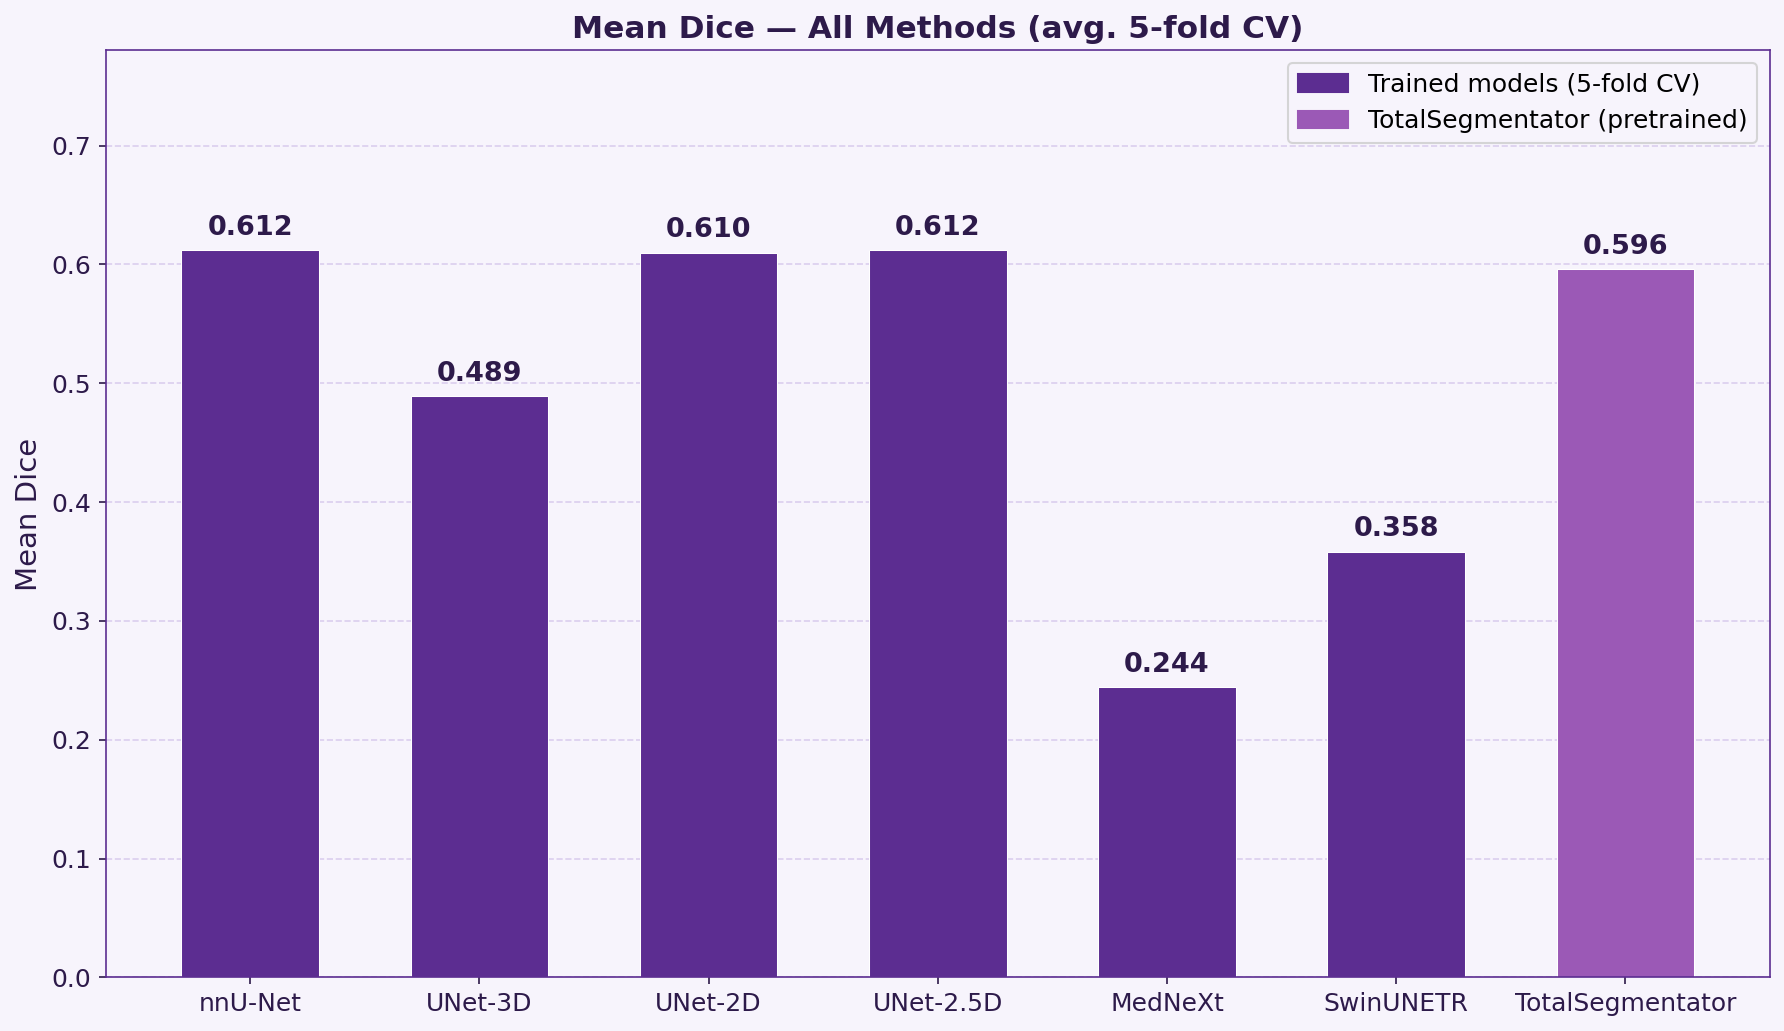
\includegraphics[width=\linewidth,height=0.52\textheight,keepaspectratio]{multiorgan_comparision2.png}
  \end{center}
}

\end{multicols}

\vspace*{\fill}

% =============================================================
% DOLNA CZĘŚĆ — pełnoszerokościowy obraz segmentacji
% =============================================================
\noindent\textcolor{pwrviolet}{\rule{\linewidth}{1.5pt}}
\vspace{2mm}

\begin{mdframed}[style=blockstyle]
  \noindent{\color{white}\colorbox{pwrviolet}{%
    \parbox{\dimexpr\linewidth-2\fboxsep\relax}{%
      \vspace{5pt}\Large\bfseries\strut
      VISUAL RESULTS — SEGMENTATION COMPARISON (CASE 66)
      \strut\vspace{5pt}}}}%
  \vspace{6pt}\par
  \begin{center}
    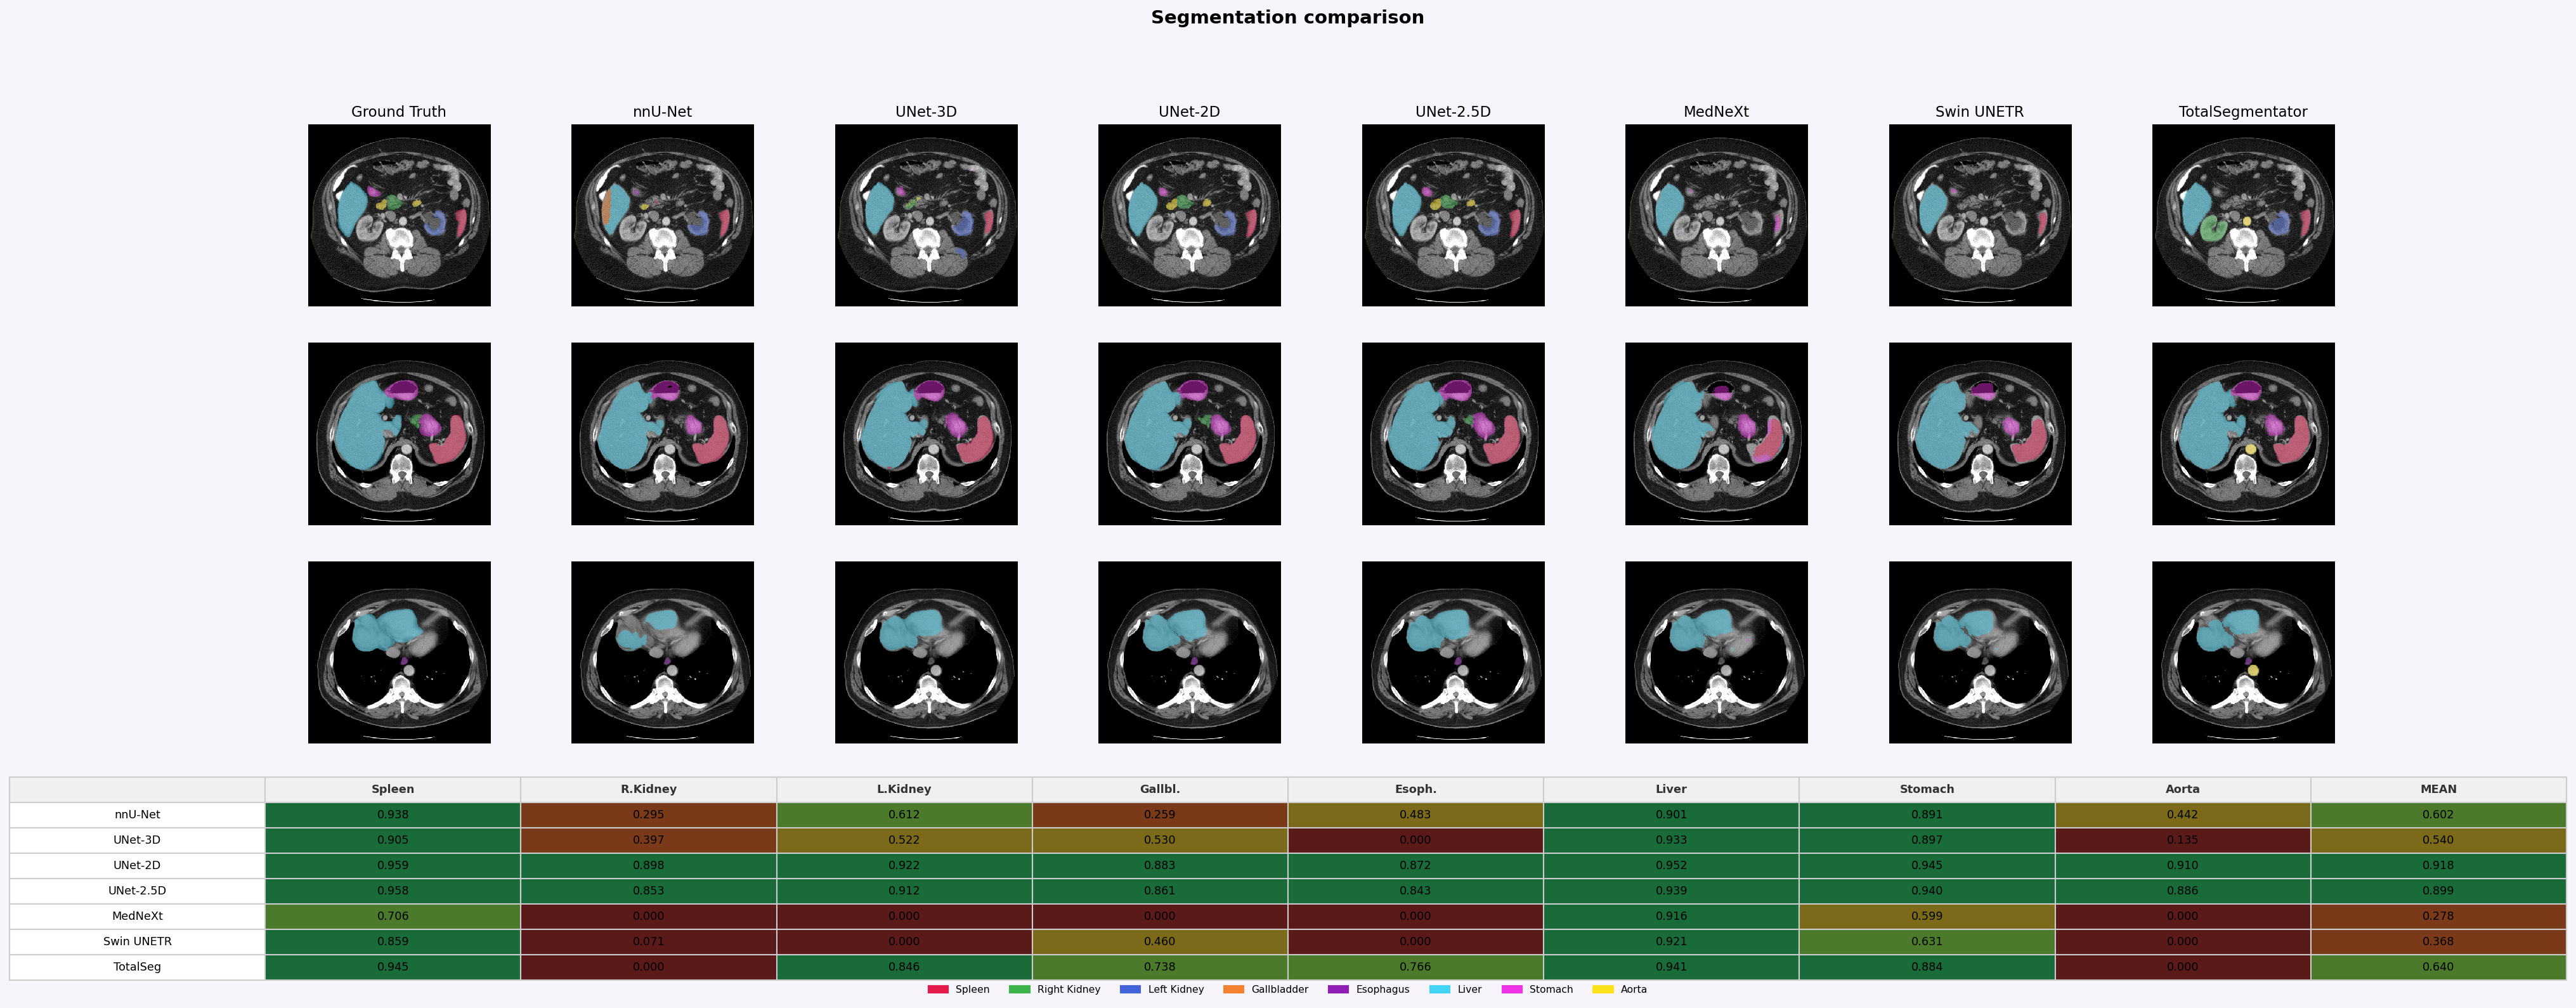
\includegraphics[width=\linewidth]{multiorgan_comparison_66.png}
  \end{center}
\end{mdframed}

\vspace*{\fill}

\end{document}
